
%(BEGIN_QUESTION)
% Copyright 2010, Tony R. Kuphaldt, released under the Creative Commons Attribution License (v 1.0)
% This means you may do almost anything with this work of mine, so long as you give me proper credit

Suppose this PLC-controlled water level system suffers a switch failure, such that the low-level switch never activates to warn the PLC of a low-level condition in the tank:

$$\includegraphics[width=15.5cm]{i04533x01.eps}$$

What operational problems will result from this switch failure?  Be as specific as you can in your answer!

\vfil 

\underbar{file i04533}
\eject
%(END_QUESTION)





%(BEGIN_ANSWER)

This is a graded question -- no answers or hints given!

%(END_ANSWER)





%(BEGIN_NOTES)

If the low-level switch fails in such a way that it never tells the PLC when there is a low level of liquid in the tank, the PLC will never know to shut off the outgoing flow (or possibly when to add additional liquid into the tank).  Thus, the possibility exists for the tank to run empty, with the drain solenoid remaining open even when it ought to close, and/or the fill solenoid remaining closed when it ought to open.

\vskip 10pt

However, you should realize that this possibility will occur {\it only if the total in-flow is less than the total out-flow through the manual ball valves.}  Otherwise, the system will actually behave normally even with the failed low-level switch.

%INDEX% Basics, control loop troubleshooting: determining effect of specified fault(s)

%(END_NOTES)

